%==============================================================================
% presentation.tex
%==============================================================================


%==============================================================================
% Configuration
%==============================================================================

% Internationalisation
\usepackage[utf8]{inputenc}
\usepackage[T1]{fontenc}
% \usepackage[ngerman]{babel}

% Different packages
\usepackage{url}
\usepackage{color,listings}
\usepackage{enumerate}
\usepackage{tabularx}
\usepackage{alltt}

% Use default Acrobat reader fonts
\usepackage{mathpazo}

% Use CM fonts (increases document size)
\usepackage{ae}

% Use images
\usepackage{graphicx}

% Configure beamer
\usetheme[secheader]{Ikhono}
\usefonttheme[onlylarge]{structurebold}
\setbeamertemplate{navigation symbols}{}

% Variables
\providecommand{\Title}{Parallel Programming}
\providecommand{\Subtitle}{Recitation Session 8}
\providecommand{\Author}{Thomas Weibel <weibelt@ethz.ch>}
\providecommand{\Institute}{Laboratory for Software Technology, \\
  Swiss Federal Institute of Technology Z\"urich}
\providecommand{\Date}{April 29, 2010}

% PDF settings
\hypersetup{
  pdftitle={\Title, \Subtitle},
  pdfauthor={\Author},
  pdfsubject={\Institute},
  pdfkeywords={parallel programming} 
}

% Titlepage
\title{\Title}
\subtitle{\Subtitle}
\author{\Author}
\institute{\Institute}
\date{\Date}

% Listings
\lstdefinestyle{Default}{
  language=Java,
  tabsize=2,
  mathescape=true,
  inputencoding=utf8,
  showstringspaces=false,
  fontadjust=true,
  basicstyle=\ttfamily,
  keywordstyle=\color{blue}\bfseries,
}
\lstset{style=Default}


%==============================================================================
% Document
%==============================================================================

\begin{document}


% Titlepage
\begin{frame}[plain]
  \titlepage
\end{frame}


\section*{Introduction}

\begin{frame}{Executive Summary}
  \begin{columns}[c]
    \begin{column}{0.6\textwidth}
      \begin{itemize}
      \item Some remarks regarding mutual exclusion proofs
      \item Repeat Read/Write locks
      \item Classroom exercise: Equivalence of Semaphores and Monitors
      \item Classroom exercise: Lock proof
      \item Implement MergeSort and Dining Philosophers with
        Communicating Sequential Processes
  \end{itemize}
      \end{column}
    \begin{column}{0.4\textwidth}
      \begin{center}
        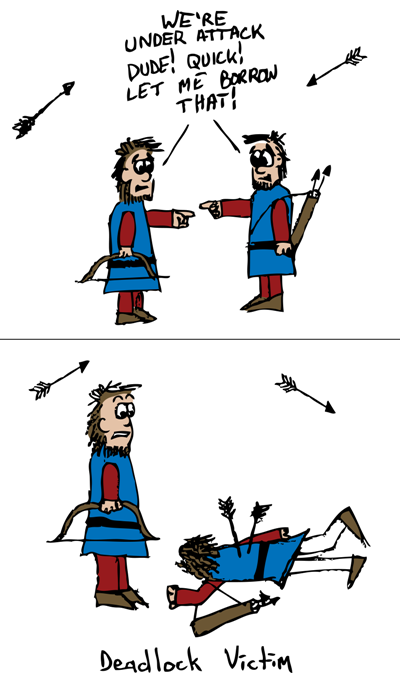
\includegraphics[width=0.9\textwidth]{figures/deadlock}\\
        \tiny{Source: \url{http://dbwhisperer.blogspot.com/2009/07/deadlocks-explained.html}}
      \end{center}
    \end{column}
  \end{columns}
\end{frame}


\section{Mutual Exclusion Proofs}

\begin{frame}{Outline}
  \tableofcontents[current]
\end{frame}

\begin{frame}[fragile]{Notation}
\begin{lstlisting}
public void run() {
  while (true) {
    mysignal.request();
    while (true) {
      if (othersignal.read() == 1) break;
      mysignal.free();
      mysignal.request();
    }
    // critical section
    mysignal.free();
  }
}
\end{lstlisting}
\end{frame}

\begin{frame}[fragile]{Notation}
  \begin{columns}[c]
    \begin{column}{0.50\textwidth}
\begin{lstlisting}[basicstyle=\fontsize{9}{11}\selectfont\ttfamily]
A1 // non-critical section
A2 turn0.flag = 0;
A3 while(true)
     if(turn1.flag == 1) 
       break;
A4   turn0.flag = 1;
A5   turn0.flag = 0;
   }
A6 // critical section
A7 turn0.flag = 1;
\end{lstlisting}
    \end{column}
    \begin{column}{0.50\textwidth}
\begin{lstlisting}[basicstyle=\fontsize{9}{11}\selectfont\ttfamily]
B1 // non-critical section
B2 turn1.flag = 0;
B3 while(true) {
     if(turn0.flag == 1) 
       break;
B4   turn1.flag = 1;
B5   turn1.flag = 0;
   }
B6 // critical section
B7 turn1.flag = 1;
\end{lstlisting}
    \end{column}
  \end{columns}
\end{frame}

\begin{frame}[fragile]{Implication}
  \begin{enumerate}
  \item \lstinline!at(A6)! $\rightarrow$ \lstinline!turn0.flag == 0!
  \end{enumerate}

  \vspace{\stretch{1}}

\begin{lstlisting}
  A1 // non-critical section
  A2 turn0.flag = 0;
  A3 while(true)
       if(turn1.flag == 1) 
         break;
  A4   turn0.flag = 1;
  A5   turn0.flag = 0;
     }
  A6 // critical section
  A7 turn0.flag = 1;
\end{lstlisting}

  \vspace{\stretch{1}}

  Why is invariant (1) true \lstinline!at(A1)!, \lstinline!at(A2)!,
  \lstinline!at(A3)!, \lstinline!at(A4)!, \lstinline!at(A5)!,
  \lstinline!at(A7)!?
\end{frame}

\begin{frame}{Implication: Truth Table}
  $$A \rightarrow B$$

  \vspace{\stretch{1}}

  \begin{center}
    \begin{tabular}{|c|c c|}
      \hline
      $\rightarrow$ & 1 & 0 \\\hline
      1 & 1 & 0 \\
      0 & 1 & 1 \\\hline
    \end{tabular}
  \end{center}

  \vspace{\stretch{1}}

  \begin{enumerate}
  \item \lstinline!at(A6)! $\rightarrow$ \lstinline!turn0.flag == 0!
  \end{enumerate}

  \vspace{\stretch{1}}

  \begin{itemize}
  \item \lstinline!at(A1)!: $0 \rightarrow x = 1$
  \item \lstinline!at(A2)!: $0 \rightarrow x = 1$
  \item \lstinline!at(A3)!: $0 \rightarrow x = 1$
  \item \lstinline!at(A4)!: $0 \rightarrow x = 1$
  \item \lstinline!at(A5)!: $0 \rightarrow x = 1$
  \item \lstinline!at(A7)!: $0 \rightarrow x = 1$
  \end{itemize}
\end{frame}

\begin{frame}[fragile]{Equivalence}
  \begin{enumerate}
  \item \lstinline!turn0.flag == 0! $\leftrightarrow$ 
    \lstinline!(at(A3) $\vee$ at(A4) $\vee$ at(A6) $\vee$ at(A7))!
  \end{enumerate}

  \vspace{\stretch{1}}

\begin{lstlisting}
  A1 // non-critical section
  A2 turn0.flag = 0;
  A3 while(true)
       if(turn1.flag == 1) 
         break;
  A4   turn0.flag = 1;
  A5   turn0.flag = 0;
     }
  A6 // critical section
  A7 turn0.flag = 1;
\end{lstlisting}

  \vspace{\stretch{1}}

  \lstinline!A4 $\rightarrow$ A5! and \lstinline!A7 $\rightarrow$ A1!:
  \lstinline!turn0.flag == 1!, why does invariant (1) still hold?
\end{frame}

\begin{frame}{Equivalence: Truth Table}
  $$A \leftrightarrow B$$

  \vspace{\stretch{1}}

  \begin{center}
    \begin{tabular}{|c|c c|}
      \hline
      $\leftrightarrow$ & 1 & 0 \\\hline
      1 & 1 & 0 \\
      0 & 0 & 1 \\\hline
    \end{tabular}
  \end{center}

  \vspace{\stretch{1}}

  \begin{enumerate}
  \item \lstinline!turn0.flag == 0! $\leftrightarrow$ 
    \lstinline!(at(A3) $\vee$ at(A4) $\vee$ at(A6) $\vee$ at(A7))!
  \end{enumerate}

  \vspace{\stretch{1}}

  \begin{itemize}  
  \item \lstinline!A4 $\rightarrow$ A5! $==$ \lstinline!at(A5)!: $0
    \leftrightarrow 0 = 1$
  \item \lstinline!A7 $\rightarrow$ A1! $==$ \lstinline!at(A1)!: $0
    \leftrightarrow 0 = 1$
  \end{itemize}
\end{frame}


\section{Read/Write Lock}

\begin{frame}{Outline}
  \tableofcontents[current]
\end{frame}

\begin{frame}{Read/Write Lock}
  \begin{itemize}
  \item Many shared objects have the property that most method calls
    return information about the object's state without modifying the
    object ({\bf readers}) while only a small number of calls actually
    modify the object ({\bf writers})
  \item There is no need for readers to synchronize with one another
    \begin{itemize}
    \item It is perfectly safe for them to access the object
      concurrently
    \end{itemize}
  \item Writers, on the other hand, must lock out readers as well as
    other writers
  \item A Read/Write Lock allows multiple readers or a single
    writer to enter the critical section concurrently
  \end{itemize}
\end{frame}

\begin{frame}{Assignment 7}
  \begin{itemize}
  \item Implement a Read/Write Lock
  \item At most four threads
  \item At most two reader threads (shared access is allowed) and one
    writer thread
  \item A thread that executes \lstinline!read()! is a reader
    \begin{itemize}
    \item At a later time it can be a writer...
    \end{itemize}
  \end{itemize}
\end{frame}

\begin{frame}[fragile]{\lstinline!Monitor!}
\begin{lstlisting}[basicstyle=\fontsize{10}{12}\selectfont\ttfamily]
public class Monitor {
  final int MAX_THREADS;
  final int MAX_READERS = 2;
  FIFOQueue waitList;
  int readers = 0;
  int writers = 0;
  boolean writing = false;
  
  public Monitor(int maxThreads) {
    MAX_THREADS = maxThreads;
    waitList = new FIFOQueue(maxThreads);
  }  
  
  public void readLock()    { /* ... */ }
  public void readUnlock()  { /* ... */ }
  public void writeLock()   { /* ... */ }
  public void writeUnlock() { /* ... */ }
}
\end{lstlisting}
\end{frame}

\begin{frame}[fragile]{\lstinline!readLock()!}
\begin{lstlisting}[basicstyle=\fontsize{7}{9}\selectfont\ttfamily]
public synchronized void readLock() {
  if (readers >= MAX_READERS || writing || !waitList.isEmpty()) {
    waitList.enq(Thread.currentThread().getId());

    while (true) {
      try {
        wait();
      } catch (InterruptedException e) {
        e.printStackTrace();
      }

      if (waitList.getFirstItem() == Thread.currentThread().getId()
          && !writing && readers < MAX_READERS) {
        waitList.deq();
        break;
      }
    }
  }

  readers++;
  if (readers < MAX_READERS)
    notifyAll();
  System.out.println("READ LOCK ACQUIRED " + readers);
}
\end{lstlisting}
\end{frame}

\begin{frame}[fragile]{\lstinline!readUnlock()!}
\begin{lstlisting}
public synchronized void readUnlock() {
  readers--;
  System.out.println("READ LOCK RELEASED " + 
                     readers);
  notifyAll();
}
\end{lstlisting}
\end{frame}

\begin{frame}[fragile]{\lstinline!writeLock()!}
\begin{lstlisting}[basicstyle=\fontsize{7}{9}\selectfont\ttfamily]
public synchronized void writeLock() {
  if (readers > 0 || writers > 0 || !waitList.isEmpty()) {
    waitList.enq(Thread.currentThread().getId());
    while (true) {
      try {
        wait();
      } catch (InterruptedException e) {
        System.out.println(e.getMessage());
      }

      if (waitList.getFirstItem() == Thread.currentThread().getId()
          && !writing && readers == 0) {
        waitList.deq();
        break;
      }
    }
  }
  
  writers++;
  writing = true;
  System.out.println("WRITE LOCK ACQUIRED " + writers);
}
\end{lstlisting}
\end{frame}

\begin{frame}[fragile]{\lstinline!writeUnlock()!}
\begin{lstlisting}
public synchronized void writeUnlock() {
  writing = false;
  writers--;    
  System.out.println("WRITE LOCK RELEASED " + 
                     writers);
  notifyAll();
}
\end{lstlisting}
\end{frame}


\section{Equivalence of Semaphores and Monitors}

\begin{frame}{Outline}
  \tableofcontents[current]
\end{frame}

\begin{frame}{Classroom Exercise}
  \begin{columns}[c]
    \begin{column}{0.45\textwidth}
      \begin{itemize}
      \item Are semaphores and monitors equivalent?
      \item How can you implement semaphores with monitors?
      \item How can you implement monitors with semaphores?
        \begin{itemize}
        \item What about \lstinline!wait()! and \lstinline!notifyAll()!?
        \end{itemize}
      \end{itemize}
    \end{column}
    \begin{column}{0.55\textwidth}
      \begin{center}
        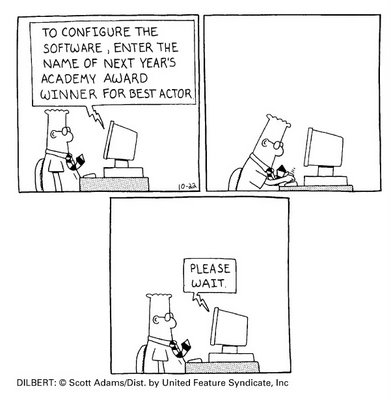
\includegraphics[width=\textwidth]{figures/dilbert-wait}
      \end{center}
    \end{column}
  \end{columns}
\end{frame}

\begin{frame}{Semaphores and Monitors}
  \begin{itemize}
  \item Monitor: model for synchronized methods in Java
  \item Both constructs are equivalent
  \item \alert{One can be used to implement the other}
  \end{itemize}
\end{frame}

\begin{frame}[fragile]{Semaphore Implementation}
\begin{lstlisting}
public class Semaphore {
  private int value;
  public Semaphore() { 
    value = 0; 
  }
  public Semaphore(int k) { 
    value = k; 
  }
  public synchronized void acquire() { 
    /* see later */ 
  }
  public synchronized void release() { 
    /* see later */ 
  }   
}
\end{lstlisting}
\end{frame}

\begin{frame}[fragile]{Semaphore Implementation: \lstinline!acquire()!}
\begin{lstlisting}
public synchronized void acquire() {
  while (value == 0) {
    try {
      wait();
    }
    catch (InterruptedException e) { 
    }
  }
  value--;
}
\end{lstlisting}
\end{frame}

\begin{frame}[fragile]{Semaphore Implementation: \lstinline!release()!}
\begin{lstlisting}
public synchronized void release() {
  ++value;
  notifyAll();
}
\end{lstlisting}
\end{frame}

\begin{frame}{Monitor with Semaphores}
  We need 2 semaphores:
  \begin{itemize}
  \item	One to make sure that only one synchronized method executes at any given time
    \begin{itemize}
    \item call this the ``access semaphore'' \lstinline!access!
    \item binary semaphore
    \end{itemize}
  \item One semaphore to line up threads that are waiting for some condition
    \begin{itemize}
    \item call this the ``condition semaphore'' \lstinline!cond!
    \item counting (general) semaphore
    \item threads that wait must do an ``acquire''
    \end{itemize}
  \end{itemize}

  \vspace{\stretch{1}}

  \begin{block}{For convenience}
    Counter \lstinline!waitThread! to count number of waiting threads
    i.e., threads in queue for \lstinline!cond!
  \end{block}  
\end{frame}

\begin{frame}{Monitor with Semaphores}
  \begin{enumerate}
  \item Frame all synchronized methods with \lstinline!access.acquire()! and
    \lstinline!access.release()!
    \begin{itemize}
    \item This ensures that only one thread executes a synchronized
      method at any point in time
    \item Recall: \lstinline!access! is binary.
    \end{itemize}
  \item Translate \lstinline!wait()! and \lstinline!notifyAll()! to give threads waiting in
    line a chance to progress (these threads use \lstinline!cond!)
  \end{enumerate}  
\end{frame}

\begin{frame}[fragile]{Monitor with Semaphores: Auxiliary Fields}
\begin{lstlisting}
class FooBar {
  private Semaphore access;
  private Semaphore cond;
  private int waitThread = 0;

  public FooBar() { 
    access = new Semaphore(1);
    cond = new Semaphore(0);
  }
  
  // continued
}
\end{lstlisting}  
\end{frame}

\begin{frame}[fragile]{(1) Framing all methods}
\begin{lstlisting}
  public void qux() {
    // Ensure mutual exclusion
    access.acquire(); 

    // Critical section

    access.release();
  }
\end{lstlisting}

  \vspace{\stretch{1}}

  is equivalent to

  \vspace{\stretch{1}}

\begin{lstlisting}
  public synchronized void qux() {
    // Critical section
  }
\end{lstlisting}
\end{frame}

\begin{frame}[fragile]{(2) Translate \lstinline!wait()!}
\begin{lstlisting}
waitThread++;

// other threads can execute 
// synchronized methods 
access.release(); 

// wait till condition changes
cond.acquire(); 
access.acquire();

waitThread--;
\end{lstlisting}
\end{frame}

\begin{frame}[fragile]{(2) Translate \lstinline!notifyAll()!}
\begin{lstlisting}
if (waitThread > 0) {
  for (int i=0; i < waitThread; i++) { 
    cond.release();
  }
}	
\end{lstlisting}

  \vspace{\stretch{1}}

  \begin{itemize}
  \item All threads waiting are released and will compete to
    (re)acquire \lstinline!access!
  \item They decrement \lstinline!waitThread! after they leave
    \lstinline!cond.acquire()!
  \item Note that to enter the line (i.e., increment
    \lstinline!waitThread!) the thread must hold the access semaphore
    \lstinline!access!
  \end{itemize}
\end{frame}

\begin{frame}{(2) Translate \lstinline!wait()! and \lstinline!notifyAll()!}
  \begin{itemize}
  \item Recall that \lstinline!access.release()! is done at the end of
    the synchronized method
  \item So all the threads that had lined up waiting for
    \lstinline!cond! compete to get access to \lstinline!access!
  \item No thread can line up while the \lstinline!cond.release()!
    operations are done since this thread holds \lstinline!access!
  \end{itemize}
\end{frame}

\begin{frame}{Note}
  \begin{itemize}
  \item We wake up all threads -- they might not be able to enter
    their critical section if the condition they waited for does not
    hold, but all threads get a chance.
  \item \lstinline!notifyAll()! calls \lstinline!cond.release()!
    \lstinline!waitThread!-times
    \begin{itemize}
    \item If 3 threads were waiting, \lstinline!cond.value! is set to 3.
    \item Now one of the threads wakes up, decrements
      \lstinline!waitThreads!, runs to the end and again calls
      \lstinline!cond.release()! 2 times $\rightarrow$
      \lstinline!cond.value! will now be 4 even though only 2 threads
      are in the wait section of the code
    \item A thread may awake a few times and not find that the
      condition has changed. As long as all the \lstinline!wait()! are
      in \lstinline!while (some_condition)! loop there will be no harm
    \end{itemize}
  \end{itemize}
\end{frame}

\begin{frame}[fragile]{\lstinline!wait()! in while-loop}
\begin{lstlisting}[basicstyle=\fontsize{9}{11}\selectfont\ttfamily]
public void insert(Object o) 
  throws InterruptedException {
  access.acquire();
  while (isFull()) {
    waitThread++;
    access.release(); // let other thread access object
    cond.acquire(); // wait for change of state
    access.acquire()
    waitThread--;
  }
  doInsert(o);	
  if (waitThread > 0) { 
    for (int i; i < waitThread; i++) {
      cond.release(); 
    } 
  }
  access.release(); 
}
\end{lstlisting}
\end{frame}


\section{Lock Proof}

\begin{frame}{Outline}
  \tableofcontents[current]
\end{frame}

\begin{frame}[fragile]{Classroom Exercise}
  \begin{columns}[c]
    \begin{column}{0.50\textwidth}
\begin{lstlisting}[basicstyle=\fontsize{9}{11}\selectfont\ttfamily]
class MyLock implements Lock {
  private int turn;
  private boolean busy = false;

  public void lock() {
    int me = ThreadID.get();
    while (turn != me) {
      while (busy) {
        turn = me;
      }
      busy = true;
    }
  }

  public void unlock() {
    busy = false;
  }
}
\end{lstlisting}
    \end{column}
    \begin{column}{0.50\textwidth}
      \begin{itemize}
      \item Does this protocol satisfy mutual exclusion?
      \item Is this protocol starvation-free?
      \item Is this protocol deadlock-free?
  \end{itemize}
    \end{column}
  \end{columns}
\end{frame}

\begin{frame}[fragile]{Lock}
\begin{lstlisting}[basicstyle=\fontsize{9}{11}\selectfont\ttfamily]
class MyLock implements Lock {
  private int turn;
  private boolean busy = false;

  public void lock() {
/* S1 */    int me = ThreadID.get();
/* S2 */    while (turn != me) {
/* S3 */      while (busy) {
/* S4 */        turn = me;
              }
/* S5 */      busy = true;
            }
  }

  public void unlock() {
/* S6 */    busy = false;
  }
}
\end{lstlisting}
\end{frame}

\begin{frame}{Mutual Exclusion}
  Protocol does not satisfy mutual exclusion:

  \vspace{\stretch{1}}

  \begin{itemize}
  \item Assume \lstinline!ThreadID!s start with a value
    \lstinline{!= 0}: \lstinline!ThreadID!s don't start with 0
    $\rightarrow$ they start with 1 in Java
  \item No thread can enter critical section (could argue this is
    mutual exclusion but you have to clarify your answer)
  \item \lstinline!turn! is initialized to 0 $\rightarrow$ one aspect
    of the broken protocol
  \end{itemize}
\end{frame}

\begin{frame}[fragile]{Mutual Exclusion}
  \lstinline!T0! attempts to enter the critical section:

  \vspace{\stretch{1}}

\begin{lstlisting}
/* S2 */ $\rightarrow$ true // me != 0
/* S3 */ false
/* S5 */ busy = true
/* S2 */ true
/* S3 */ true // bye virtue of S5, 
              // previous iteration
/* S4 */ turn = me
/* S3 */ true // no exit from loop
\end{lstlisting}

  \vspace{\stretch{1}}

  If another thread attempts to enter the critical section then it
  will experience the same sequence
\end{frame}

\begin{frame}[fragile]{Mutual Exclusion}
  \begin{itemize}
  \item Assume that \lstinline!ThreadID!s start at 0 or
    \lstinline!turn! is initialized to the \lstinline!ThreadID! of the
    first thread (i.e. 1) to enter the critical section
  \item This thread succeeds but does not set \lstinline!busy! to
    true:
\begin{lstlisting}
/* S1 */   me = 0 // by assumption
/* S2 */   $\rightarrow$ false
\end{lstlisting}
    Loop exits but \lstinline!busy! unchanged (\lstinline!false!)
  \end{itemize}
\end{frame}

\begin{frame}{Starvation}
  \begin{itemize}
  \item Protocol is not starvation-free
  \item Assume there are two threads:
    \begin{itemize}
    \item If \lstinline!turn! is not initialized to the
      \lstinline!ThreadID! of the first thread to acquire the lock,
      then this thread will be not able to enter its critical section
    \item If \lstinline!turn! is initialized then the second thread
      never enters its critical section if the first thread leaves its
      critical section (with \lstinline!unlock()!) before the second
      thread attempts to enter its critical section
    \end{itemize}
  \end{itemize}
\end{frame}

\begin{frame}{Deadlock}
  \begin{itemize}
  \item Protocol is not deadlock-free
  \item Situation for deadlock is similar to the situation for
    starvation in this case
  \item The thread will enter the lock method but never exit
  \end{itemize}
\end{frame}


\section{JCSP: Semaphores}

\begin{frame}{Outline}
  \tableofcontents[current]
\end{frame}

\begin{frame}[fragile]{Semaphores}
  \begin{itemize}
  \item Special Integer variable with 2 atomic operations
    \begin{itemize}
    \item \lstinline!P()!: Passeren, wait/up
    \item \lstinline!V()!: Vrijgeven/Verhogen, signal/down
    \end{itemize}
  \item Map into JCSP by defining a semaphore process
  \end{itemize}
\end{frame}

\begin{frame}{Semaphores in JCSP}
  \begin{itemize}
  \item Semaphore \lstinline!CSProcess!
  \item Two channels for \lstinline!P! and \lstinline!V!
  \item Two + Two channels
    \begin{itemize}
    \item \lstinline!P! -- request/confirm
    \item \lstinline!V! -- request/confirm
    \end{itemize}
  \end{itemize}
\end{frame}


\section{JCSP: MergeSort}

\begin{frame}{Outline}
  \tableofcontents[current]
\end{frame}

\begin{frame}{Overview}
  \begin{itemize}
  \item Thread hierarchy similar to previous mergesort assignment
  \item Threads are replaced with JCSP processes
  \item Communication allowed only via JCSP channels – no shared data
    between processes
  \item Use the JCSP library provided on the website
  \end{itemize}
\end{frame}

\begin{frame}{Entities Description}
  \begin{description}
  \item[Sorting process:] randomly generates a subarray, sorts it
    sequentially, and then passes the result to its parent merging
    process
  \item[Merging process:] takes 2 sorted subarrays from its children,
    merges and passes the result to its parent merging process
  \item[Communication channel:] allows data passing between processes
  \end{description}
\end{frame}

\begin{frame}{Entities Layout}
  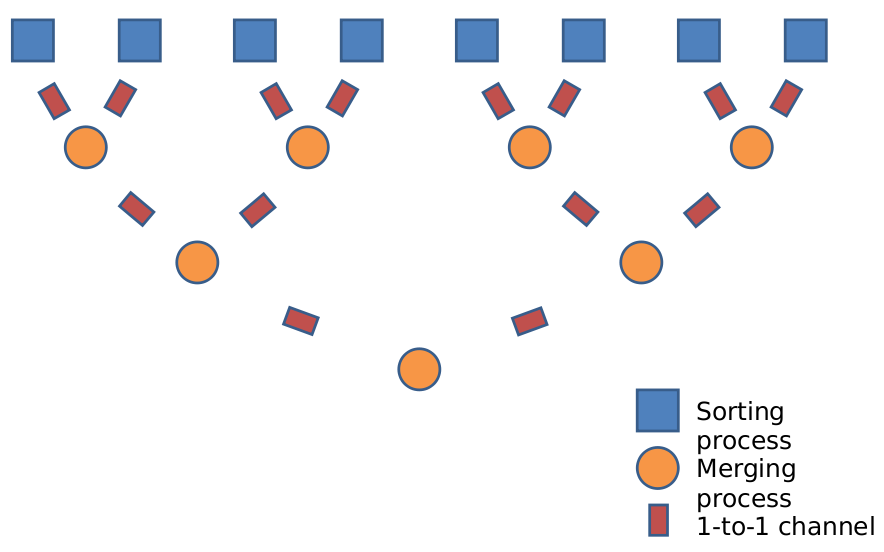
\includegraphics[width=\textwidth]{figures/mergesort}
\end{frame}

\begin{frame}{Reading Policy}
  How can the data from 2 children be read?

  \vspace{\stretch{1}}

  \begin{enumerate}
  \item Read all data from first child, then read all data from second
    child
   \begin{itemize}
   \item Read whole subarray
   \end{itemize}
 \item Read data from both children simultaneously
   \begin{itemize}
   \item Read whole subarray
   \end{itemize}
 \item Similar to (2), but read data in pairs and proceed to output
   current element of the not-yet-fully-sorted subarray
   \begin{itemize}
   \item Read subarray element-wise
   \end{itemize}

  \end{enumerate}
\end{frame}

\begin{frame}[fragile]{Skeleton}
\begin{lstlisting}[basicstyle=\fontsize{7}{9}\selectfont\ttfamily]
import org.jcsp.lang.*;

public class MergeSort {
  // TODO: add possible fields and methods
  
  public static void main(String[] args) {
    // the total number of JCSP processes that will be run 
    // (will be changed, of course, by your code)
    int numberOfProcesses = 0;
    
    // TODO: add code here
    
    // create process array
    CSProcess[] allProcesses = new CSProcess[numberOfProcesses];
    
    // TODO: add code here
    
    // run all JCSP processes, they should synchronize via the 
    // communication channels
    Parallel parallel = new Parallel(allProcesses);
    parallel.run();
  }
}
\end{lstlisting}
\end{frame}

\begin{frame}[fragile]{Skeleton: Sorting}
\begin{lstlisting}[basicstyle=\fontsize{9}{11}\selectfont\ttfamily]
import java.util.Random;
import org.jcsp.lang.*;

public class SortingProcess implements CSProcess {
  // TODO: add possible fields/methods
  
  public SortingProcess() {
    // TODO: add code, change signature if necessary
  }
    
  public void run() {
    // TODO: initialize random subarray (or do it in
    //       the constructor, alternatively), sort
    //       it sequentially, and write it to parent
   }
}
\end{lstlisting}
\end{frame}

\begin{frame}[fragile]{Skeleton: Merging}
\begin{lstlisting}[basicstyle=\fontsize{9}{11}\selectfont\ttfamily]
import org.jcsp.lang.*;

public class MergingProcess implements CSProcess {
  // TODO: add possible fields/methods
  
  public MergingProcess() {
    // TODO: add code, change signature if necessary
  }
  
  // the process' run() method
  public void run() {
    // TODO: read subarrays from children, merge them, 
    //       write merged subarray to parent
  }
}
\end{lstlisting}
\end{frame}


\section{JCSP: Dining Philosophers}

\begin{frame}{Outline}
  \tableofcontents[current]
\end{frame}

\begin{frame}{Dining Philosophers}
  \begin{center}
    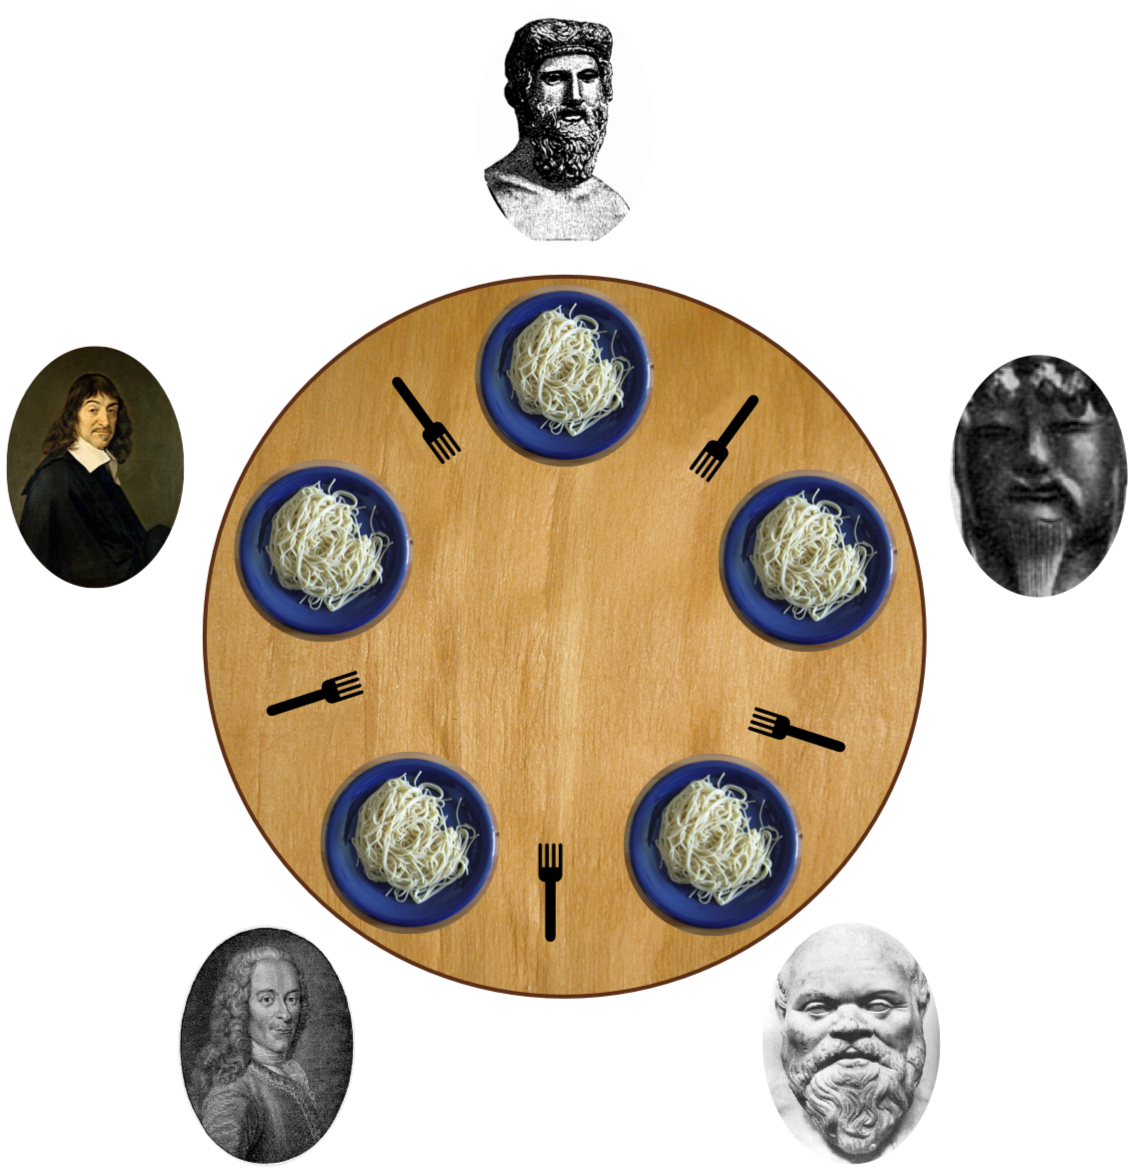
\includegraphics[width=0.65\textwidth]{figures/dining-philosophers} \\
    \tiny{Source: \url{http://en.wikipedia.org/wiki/File:Dining_philosophers.png}}
  \end{center}
\end{frame}

\begin{frame}{Dining Philosophers}
  \begin{itemize}
  \item Five philosophers sitting at a table doing one of two things:
    \begin{itemize}
    \item eating or
    \item thinking
    \end{itemize}
  \item While eating, they are not thinking, and while thinking, they
    are not eating
  \item Philosophers sit at a circular table with a large bowl of
    spaghetti in the center
  \item Each philosopher has one fork to his left and one fork to his
    right
  \item Philosopher must eat with two forks: Can only use the forks on
    his immediate left and immediate right
  \end{itemize}
\end{frame}

\begin{frame}{Deadlock and Starvation}
  \begin{block}{Deadlock}
    Philosophers never speak to each other: creates a dangerous
    possibility of deadlock when every philosopher holds a left fork
    and waits perpetually for a right fork (or vice versa)
  \end{block}

  \begin{center}
    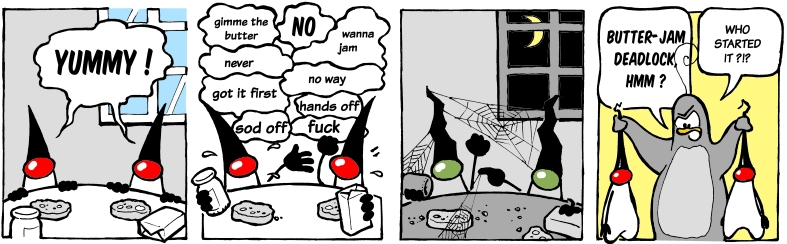
\includegraphics[width=0.85\textwidth]{figures/butter-jam-deadlock}
  \end{center}

  \begin{block}{Starvation}
    Starvation -- pun intended -- might also occur independently of
    deadlock if a philosopher is unable to acquire both forks because
    of a timing problem
  \end{block}
\end{frame}

\begin{frame}{Strategies to Avoid Deadlock}
  \begin{columns}[c]
    \begin{column}{0.45\textwidth}
  \begin{itemize}
  \item Security Guard: limits entry to dining hall
  \item Asymmetric philosophers: 4 philosophers pick up left fork
    first, 1 philosopher picks up right fork first
  \item See \url{http://en.wikipedia.org/wiki/Dining_philosophers_problem\#Solutions} 
    for other strategies
  \end{itemize}
    \end{column}
    \begin{column}{0.55\textwidth}
      \begin{center}
        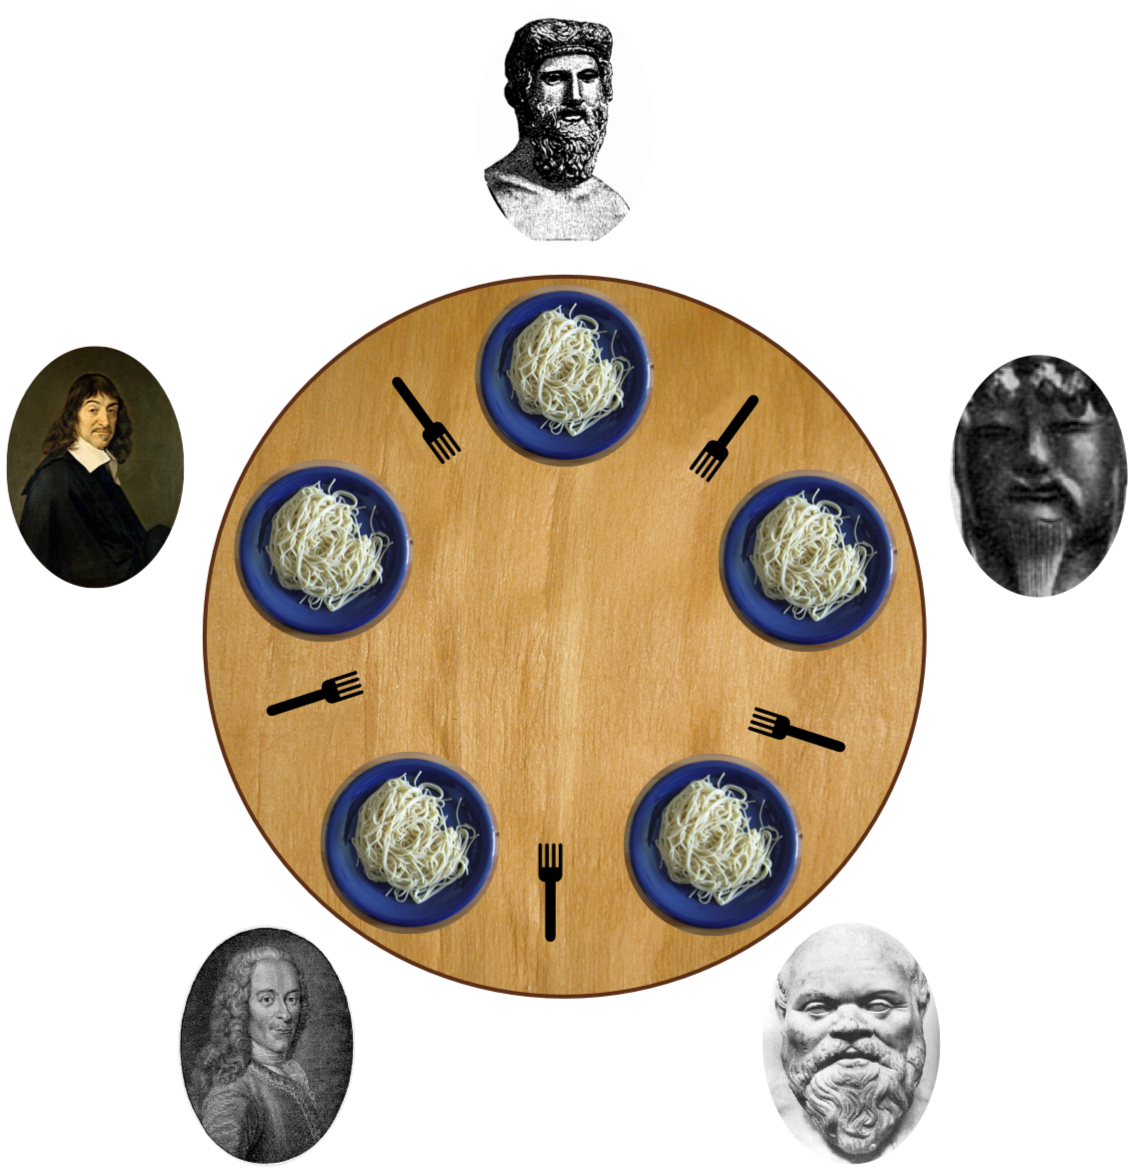
\includegraphics[width=\textwidth]{figures/dining-philosophers} \\
        \tiny{Source: \url{http://en.wikipedia.org/wiki/File:Dining_philosophers.png}}
      \end{center}
    \end{column}
  \end{columns}
\end{frame}

\begin{frame}[fragile]{Skeleton: Main}
\begin{lstlisting}[basicstyle=\fontsize{7}{9}\selectfont\ttfamily]
import org.jcsp.lang.CSProcess;
import org.jcsp.lang.Parallel;

public class Main implements CSProcess {
  private final static int NUM_PHILOSOPHERS = 5;
  private final CSProcess go;

  public Main() {
    final Philosopher[] philosophers = new Philosopher[NUM_PHILOSOPHERS];
    for (int i = 0; i < philosophers.length; i++) {
      philosophers[i] = new Philosopher(i);
    }
    go = new Parallel(new CSProcess[] {new Parallel(philosophers)});
  }

  @Override
  public void run() {
    go.run();
  }

  public static void main(String[] args) {
    new Main().run();
  }
}
\end{lstlisting}
\end{frame}

\begin{frame}[fragile]{Skeleton: Philosopher}
\begin{lstlisting}[basicstyle=\fontsize{6}{8}\selectfont\ttfamily]
import org.jcsp.lang.CSProcess;

public class Philosopher implements CSProcess {
  private final int ID;
  public Philosopher(int id) {
    this.ID = id;
  }

  @Override
  public void run() {
    try {
      for (;;) {
        think(); eat();      
      }
    } catch (InterruptedException e) {
      e.printStackTrace();
    }
  }
  private void think() throws InterruptedException { 
    Thread.sleep((long)(Math.random() * 500));
    System.out.println("Philosopher " + ID + " : Thinking...");
  }
  private void eat() throws InterruptedException {
    Thread.sleep((long)(Math.random() * 500));
    System.out.println("Philosopher " + ID + " : Please, give me two forks!");
  }
}
\end{lstlisting}
\end{frame}


\section*{Outro}

\begin{frame}{Summary}
  \begin{itemize}
  \item Mutual exclusion proofs
  \item Read/Write locks
  \item Equivalence of Semaphores and Monitors
  \item Lock proof
  \item MergeSort and Dining Philosophers in JCSP
  \end{itemize}

  \vspace{\stretch{1}}

  \begin{center}
    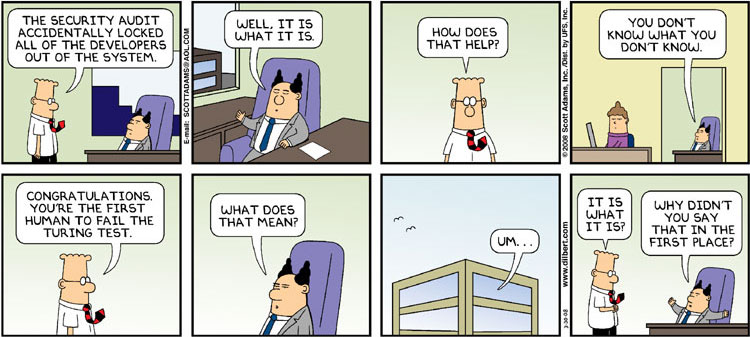
\includegraphics[scale=0.4]{figures/dilbert-turing-test}
  \end{center}
\end{frame}

\end{document}
